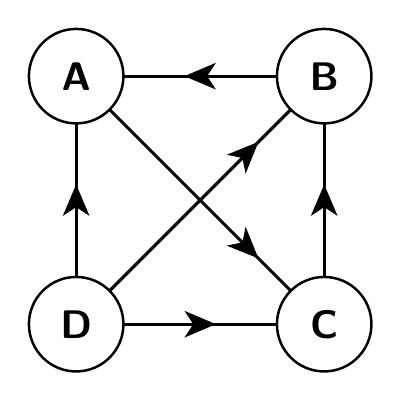
\begin{tikzpicture}[x=1cm,y=1cm]
\draw[line width=1.1pt] (0,0.6) -- (0,2.55);
\draw[line width=1.1pt] (0.424,0.424) -- (2.726,2.726);
\draw[line width=1.1pt] (0.6,0) -- (2.55,0);
\draw[line width=1.1pt] (0.424,2.726) -- (2.726,0.424);
\draw[line width=1.1pt] (3.15,0.6) -- (3.15,2.55);
\draw[line width=1.1pt] (2.55,3.15) -- (0.6,3.15);
\fill[black] (0,1.775) -- (-0.17,1.375) -- (0,1.487) -- (0.17,1.375) -- cycle;
\fill[black] (2.315,2.315) -- (1.912,2.152) -- (2.111,2.111) -- (2.152,1.912) -- cycle;
\fill[black] (1.775,0) -- (1.375,0.17) -- (1.487,0) -- (1.375,-0.17) -- cycle;
\fill[black] (2.315,0.835) -- (2.152,1.238) -- (2.111,1.039) -- (1.912,0.998) -- cycle;
\fill[black] (3.15,1.775) -- (2.98,1.375) -- (3.15,1.487) -- (3.32,1.375) -- cycle;
\fill[black] (1.375,3.15) -- (1.775,2.98) -- (1.663,3.15) -- (1.775,3.32) -- cycle;
\filldraw[fill=white, line width=0.9pt] (0,3.15) circle (0.6);
\node[font=\sffamily\bfseries\Large] at (0,3.15) {A};
\filldraw[fill=white, line width=0.9pt] (3.15,3.15) circle (0.6);
\node[font=\sffamily\bfseries\Large] at (3.15,3.15) {B};
\filldraw[fill=white, line width=0.9pt] (3.15,0) circle (0.6);
\node[font=\sffamily\bfseries\Large] at (3.15,0) {C};
\filldraw[fill=white, line width=0.9pt] (0,0) circle (0.6);
\node[font=\sffamily\bfseries\Large] at (0,0) {D};
\end{tikzpicture}
